% RMA（Kumar et al., RSS 2021）の論文紹介．
% コンパイル（slide/others/ で実行。PDFは slide/out/others/ 、他は build/）:
%   ../lualatex-dated.sh -interaction=nonstopmode -output-directory=out rma_legged_robot_ja.tex
\documentclass[aspectratio=169,10pt,t]{beamer}
\usepackage[ja]{labslide}

\graphicspath{{../../paper_tex/rma_legged_robot/figures/}}

\kicker{論文紹介}
\title[RMA：脚ロボットの高速な運動適応]{RMA：脚ロボットの高速な運動適応}
\subtitle{未経験の地面や荷物に，1秒未満で歩き方を合わせる}
\author{Ashish Kumar, Zipeng Fu, Deepak Pathak, Jitendra Malik}
\venue{RSS 2021 \quad UC Berkeley / Carnegie Mellon University}
\date{2026年9月}

\begin{document}

\begin{frame}[plain]
  \labtitlepage{%
    \agendacard[blue]{実時間で適応する}{転ぶ前に，歩き方を変える．}%
    \hfill
    \agendacard[orange]{方策と推定を分ける}{学習はシミュレーションで終える．}%
    \hfill
    \agendacard[green]{未知の地形を歩く}{校正も実機学習も使わない．}%
  }
\end{frame}

\begin{frame}{問題 ｜ 歩きながら，その場で合わせる}
  {\footnotesize\color{muted} 合わせる対象：砂，泥，草，段差，滑る床，荷物}

  \vspace{1.15em}
  \begin{columns}[T,onlytextwidth]
    \begin{column}{0.48\textwidth}
      \infocard[orange]{RMA の適応}{1秒未満．歩きながら，その場で歩き方を変える．学習はシミュレーションで終え，実機では追加の試行をしない．}
    \end{column}
    \hfill
    \begin{column}{0.48\textwidth}
      \infocard[blue]{Peng et al.\ (2020)}{実機の上で 4--8 分．まだ歩けない状態でデータを集めると，転倒になり，機体を痛める．}
    \end{column}
  \end{columns}

  \takeaway{基本の歩き方に加え，適応のしかたもシミュレーションで学び，実機はそのまま使う．}
  \source{Kumar et al., RSS 2021, §1}
\end{frame}

\begin{frame}{背景 ｜ シミュレータと実世界のずれは重なる}
  \begin{columns}[T,onlytextwidth]
    \begin{column}{0.32\textwidth}
      \infocard[blue]{機体とモデル}{シミュレータの形と，実機の機体が違う．}
    \end{column}
    \hfill
    \begin{column}{0.32\textwidth}
      \infocard[orange]{地形の多様性}{実地は，訓練に置いた地形モデルより広い．}
    \end{column}
    \hfill
    \begin{column}{0.32\textwidth}
      \infocard[green]{接触と変形}{沈む地面や接触は，剛体シミュレータが苦手．}
    \end{column}
  \end{columns}

  \vspace{1.1em}
  \centering
  {\footnotesize\color{muted} 推定用のデータを，どこで集めるか}\\[0.55em]
  \begin{tikzpicture}[node distance=5mm]
    \node[kwblue, text width=26mm] (a) {実機で\\4--8分};
    \node[kwblue, text width=26mm, right=of a] (b) {パラメータ\\を推定};
    \draw[kwarr] (a) -- (b);
    \node[kworange, text width=28mm, right=12mm of b] (c) {履歴は\\シミュレータ};
    \node[kworange, text width=24mm, right=of c] (d) {$\phi$ を\\訓練};
    \draw[kwarr] (c) -- (d);
    \node[font=\scriptsize, text=muted, above=1.4mm of a] {これまでの適応};
    \node[font=\scriptsize, text=muted, above=1.4mm of c] {RMA};
  \end{tikzpicture}

  \takeaway{適応用のデータ収集を実機に置かない．推定器もシミュレーションで訓練する．}
  \source{Kumar et al., §1 \quad Peng et al., RSS 2020}
\end{frame}

\begin{frame}{関連研究 ｜ 頑健さ，同定，実機での追加学習}
  \begin{columns}[T,onlytextwidth]
    \begin{column}{0.32\textwidth}
      \infocard[blue]{モデルベース制御}{正確な動力学と，歩容の手調整．Cheetah 3 の MPC や，ANYmal の倒立振子計画．}
    \end{column}
    \hfill
    \begin{column}{0.32\textwidth}
      \infocard[orange]{環境のランダム化}{摩擦や質量をばらして頑健にする．その範囲では保守的な歩き方になりやすい．}
    \end{column}
    \hfill
    \begin{column}{0.32\textwidth}
      \infocard[green]{実機での同定}{潜在変数を実機の試行で最適化する．初期化が速くても，複数回の試行が残る．}
    \end{column}
  \end{columns}

  \takeaway{RMA は特権情報で歩き方を学び，実行時はその代わりに直近の履歴を使う．}
  \source{Kumar et al., §2 \quad Lee et al.\ (2020) は実機で頑健だが，軌道生成器とモータモデルを手で与える．}
\end{frame}

\begin{frame}{手法 ｜ 学習時だけ環境を見せ，実行時は履歴で補う}
  \centering
  \begin{tikzpicture}[node distance=3.6mm]
    \node[kwgreen, text width=20mm] (e) {環境\\$e_t$};
    \node[kwgreen, text width=20mm, right=of e] (mu) {符号化器\\$\mu$};
    \node[kwgreen, text width=20mm, right=of mu] (z) {潜在変数\\$z_t$};
    \node[kwgreen, text width=20mm, right=of z] (pi) {方策\\$\pi$};
    \node[kwgreen, text width=20mm, right=of pi] (a) {関節目標\\$a_t$};
    \draw[kwarr] (e) -- (mu);
    \draw[kwarr] (mu) -- (z);
    \draw[kwarr] (z) -- (pi);
    \draw[kwarr] (pi) -- (a);
    \node[font=\scriptsize, text=muted, anchor=south west]
      at ([yshift=1.6mm]e.north west)
      {第1段階：強化学習．$e_t$ はシミュレーションの中だけで既知};

    \node[kworange, text width=20mm, below=10mm of e] (h) {0.5秒の\\履歴};
    \node[kworange, text width=20mm, right=of h] (phi) {適応器\\$\phi$};
    \node[kworange, text width=20mm, right=of phi] (zh) {推定\\$\hat z_t$};
    \node[kworange, text width=20mm, right=of zh] (pi2) {同じ方策\\$\pi$};
    \node[kworange, text width=20mm, right=of pi2] (a2) {関節目標\\$a_t$};
    \draw[kwarr] (h) -- (phi);
    \draw[kwarr] (phi) -- (zh);
    \draw[kwarr] (zh) -- (pi2);
    \draw[kwarr] (pi2) -- (a2);
    \node[font=\scriptsize, text=muted, anchor=south west]
      at ([yshift=1.6mm]h.north west)
      {第2段階と実行時：履歴から $\hat z_t$ を当て，同じ $\pi$ に渡す};
  \end{tikzpicture}

  \takeaway{実機に無い $e_t$ は学習時だけ使い，実行時は状態と行動の履歴から $z_t$ を復元する．}
  \source{Kumar et al., Fig.~2 / §3}
\end{frame}

\begin{frame}{手法 ｜ 原著の二段階と，実機での二つの周期}
  \centering
  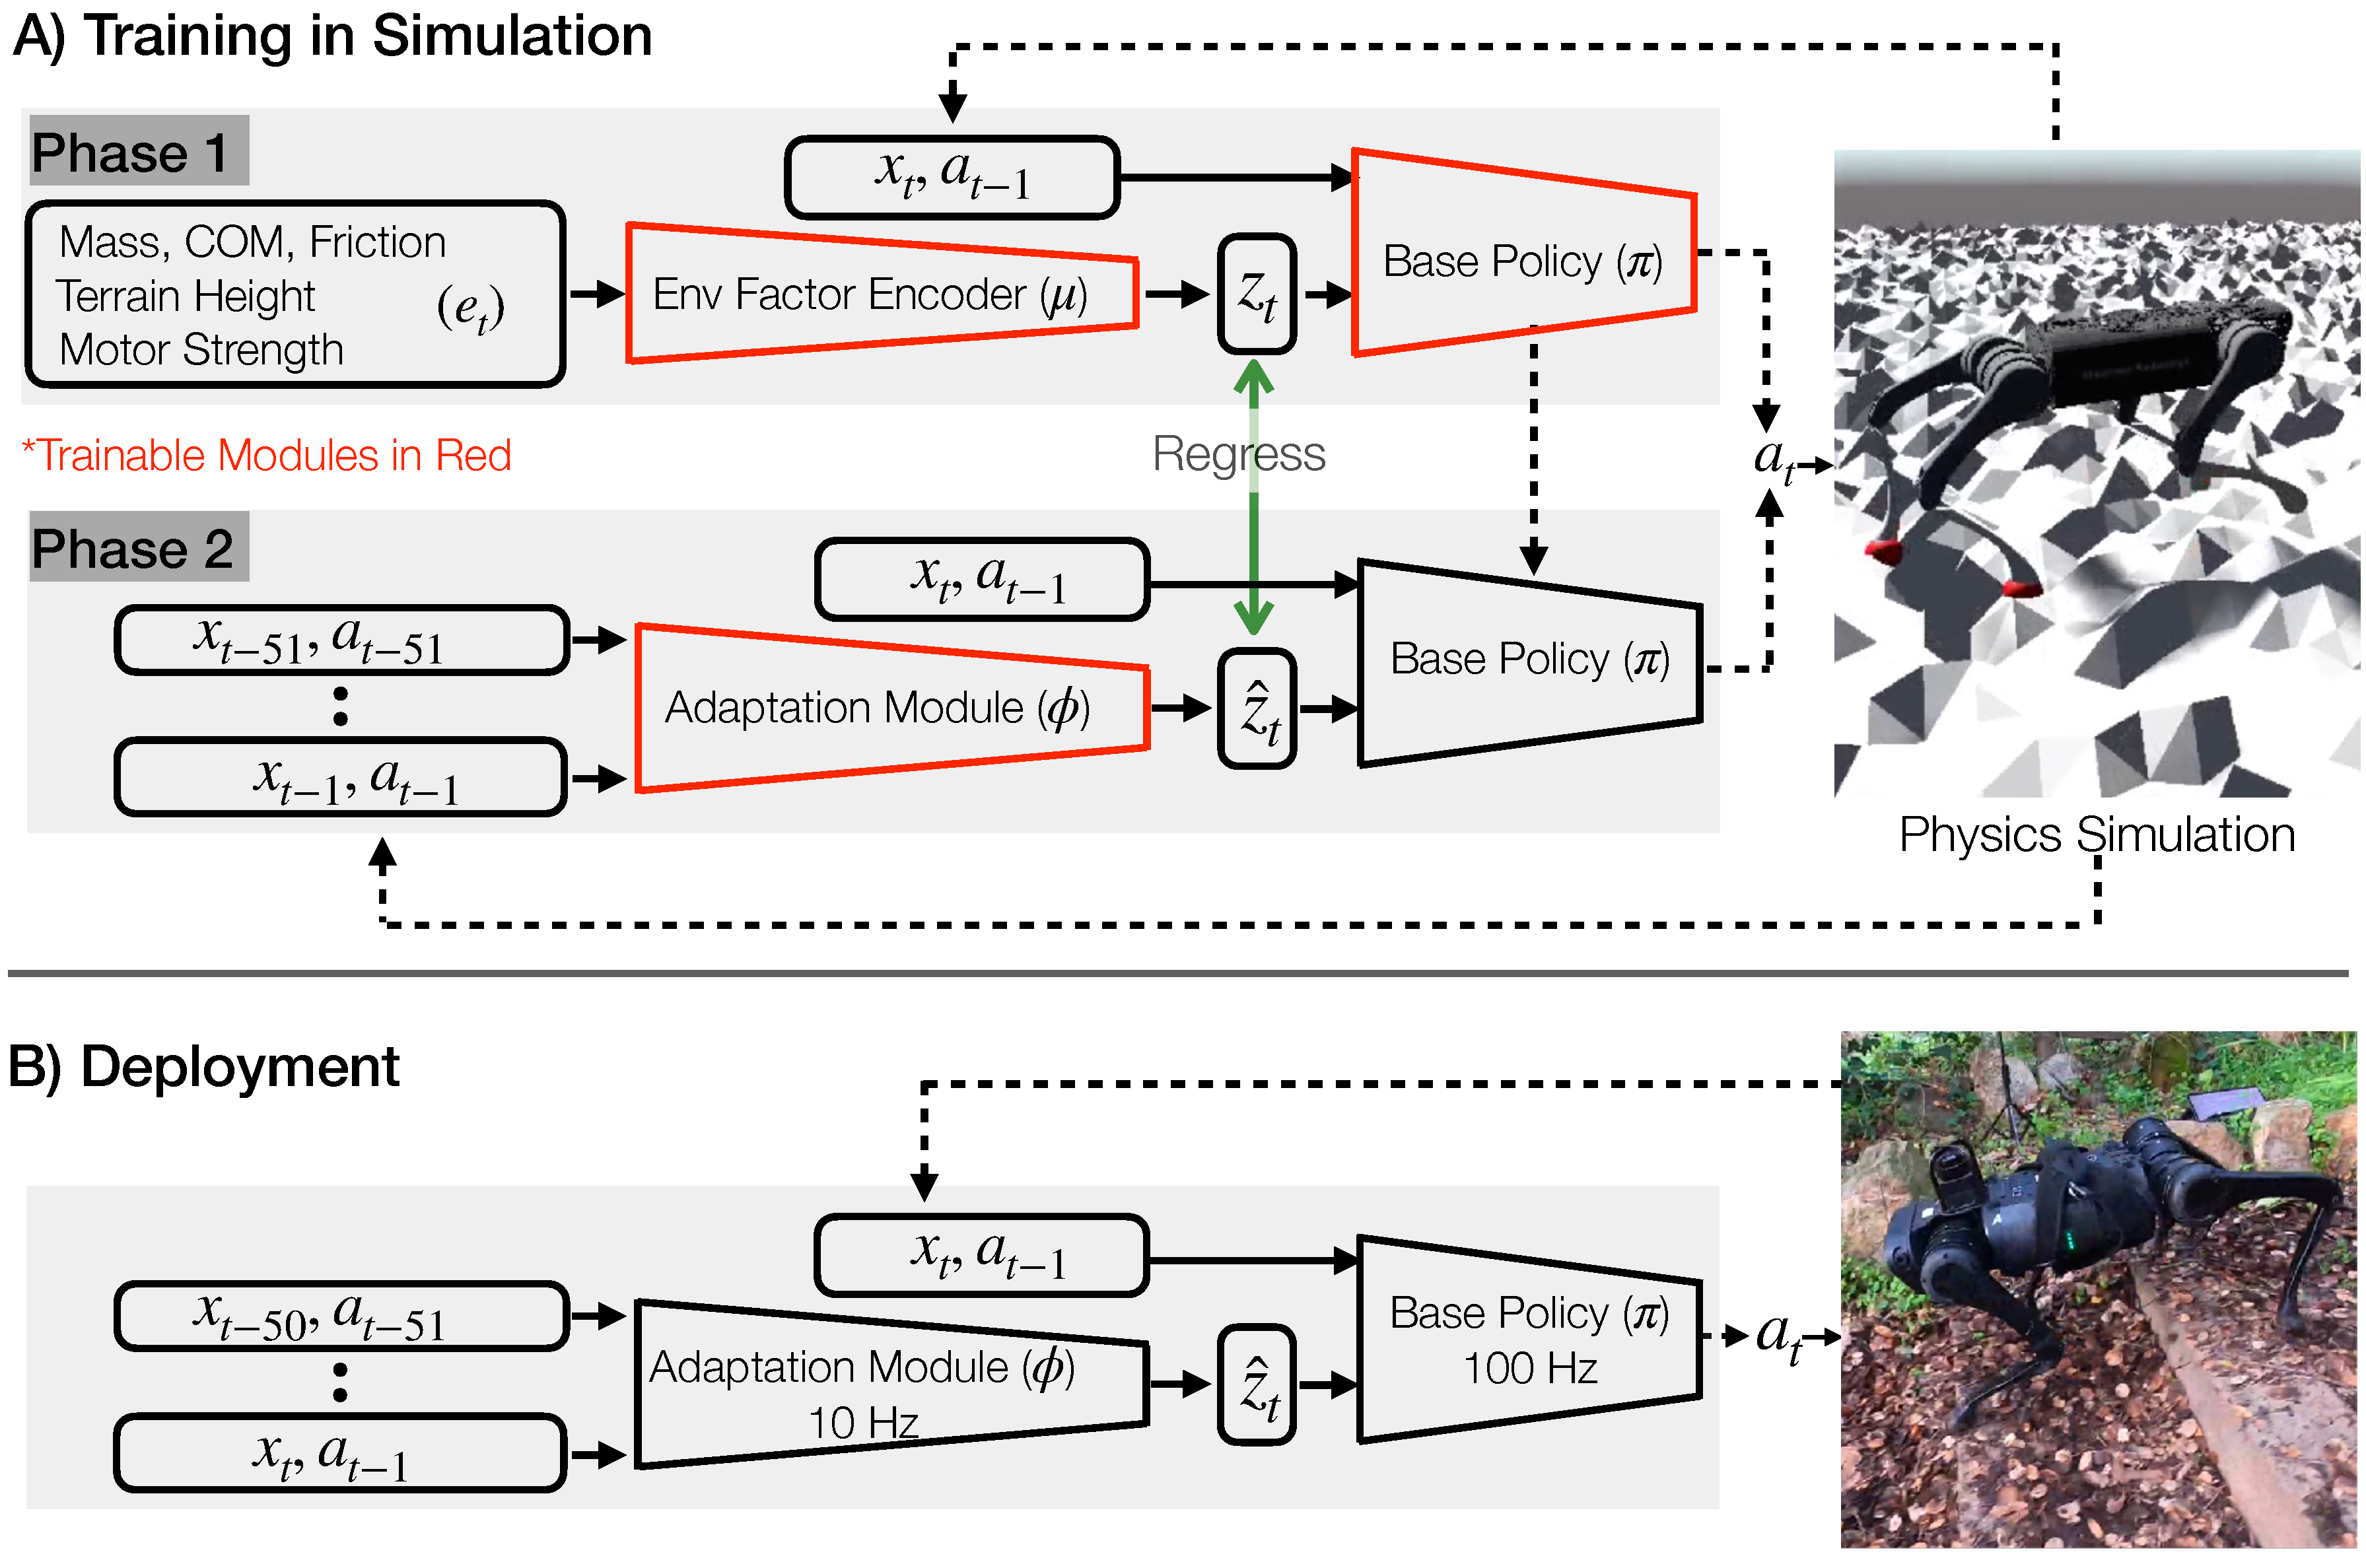
\includegraphics[height=56mm,keepaspectratio]{rma-method-1.pdf}

  \vspace{1.0mm}
  \raggedright
  {\scriptsize\color{muted}
  原著 Fig.~2．赤枠が学習する部品．上段がシミュレーションでの二段階，下段が実機．$\phi$ は 10\,Hz，$\pi$ は 100\,Hz．}
\end{frame}

\begin{frame}{第1段階 ｜ 環境が分かっているつもりで歩く}
  \centering
  {\small $z_t = \mu(e_t)\in\mathbb{R}^{8}$\quad $\rightarrow$\quad $a_t = \pi(x_t, a_{t-1}, z_t)$}

  \vspace{0.7em}
  \begin{columns}[T,onlytextwidth]
    \begin{column}{0.32\textwidth}
      \infocard[blue]{$e_t$：17次元}{質量と重心 3\\モータ強度 12\\摩擦 1，地形高さ 1}
    \end{column}
    \hfill
    \begin{column}{0.32\textwidth}
      \infocard[orange]{$x_t$：30次元}{関節の位置と速度\\胴体の roll / pitch\\足の接触}
    \end{column}
    \hfill
    \begin{column}{0.32\textwidth}
      \infocard[green]{$a_t$：12次元}{12関節の目標角度\\PD でトルクへ\\$K_p=55$，$K_d=0.8$}
    \end{column}
  \end{columns}

  \vspace{0.85em}
  \metricbox[green]{15{,}000}{PPO の iteration}\hspace{1.1em}%
  \metricbox[green]{約24時間}{1台のデスクトップ}\hspace{1.1em}%
  \metricbox[green]{12億}{シミュレータのステップ}

  \takeaway{$z_t$ は摩擦や質量の写しではなく，歩き方をどう変えるかの要約である．}
  \source{Kumar et al., §3.1, §4.2}
\end{frame}

\begin{frame}{第1段階 ｜ 見本の歩容は与えない}
  \begin{columns}[T,onlytextwidth]
    \begin{column}{0.34\textwidth}
      \infocard[orange]{見本は与えない}{前方速度の上限は 0.35\,m/s．参照する歩容は無い．}
    \end{column}
    \hfill
    \begin{column}{0.63\textwidth}
      \infocard[blue]{罰する量}{横移動，旋回，仕事，着地衝撃．トルクの急変，大きな行動，関節速度．姿勢の傾き，上下加速度，足の滑り．}
    \end{column}
  \end{columns}

  \vspace{1.15em}
  \centering
  {\footnotesize\color{muted} カリキュラム}\\[0.55em]
  \begin{tikzpicture}[node distance=6mm]
    \node[kwgreen, text width=32mm] (p) {罰は\\弱く始める};
    \node[kwgreen, text width=34mm, right=of p] (q) {係数とばらつき\\を上げる};
    \node[kwgreen, text width=34mm, right=of q] (r) {地形は最初から\\フラクタル};
    \draw[kwarr] (p) -- (q);
    \draw[kwarr] (q) -- (r);
  \end{tikzpicture}

  \takeaway{仕事と着地衝撃に寄せた報酬と，凸凹の地形で，参照軌道なしの歩容を作る．}
  \source{Kumar et al., §3.1}
\end{frame}

\begin{frame}{第2段階 ｜ 直近 0.5 秒から $z_t$ を推定する}
  \centering
  {\small $\hat z_t = \phi(x_{t-50:t-1}, a_{t-50:t-1})$}
  \quad{\footnotesize\color{muted} 50ステップ $=$ 0.5秒 \quad 1次元 CNN \quad MSE}

  \vspace{0.85em}
  \begin{columns}[T,onlytextwidth]
    \begin{column}{0.48\textwidth}
      \infocard[blue]{真の $z_t$ だけで集める}{残るのは成功した歩きだけ．崩れた歩容を $\phi$ が知らない．}
    \end{column}
    \hfill
    \begin{column}{0.48\textwidth}
      \infocard[orange]{RMA：$\hat z_t$ で集める}{崩れた履歴も入る．真の $z_t$ との MSE で $\phi$ を更新する．}
    \end{column}
  \end{columns}

  \vspace{0.9em}
  \centering
  {\footnotesize\color{muted} 1{,}000 iteration \quad 約 3 時間 \quad 8{,}000 万ステップ}

  \takeaway{当てるのは摩擦の数値ではなく方策が使う $z_t$ なので，完全なシステム同定は要らない．}
  \source{Kumar et al., §3.2}
\end{frame}

\begin{frame}{実行 ｜ 遅い推定と速い制御を，時計を揃えずに走らせる}
  \centering
  \begin{tikzpicture}[node distance=8mm]
    \node[kwgreen, text width=32mm] (phi) {適応器 $\phi$\\10\,Hz\\履歴 0.5秒};
    \node[kwgreen, text width=32mm, right=of phi] (pi) {方策 $\pi$\\100\,Hz\\最新の $\hat z_t$};
    \node[kwgreen, text width=26mm, right=of pi] (a) {関節目標\\$a_t$};
    \draw[kwarr] (phi) -- (pi);
    \draw[kwarr] (pi) -- (a);
  \end{tikzpicture}

  \vspace{0.7em}
  \begin{columns}[T,onlytextwidth]
    \begin{column}{0.48\textwidth}
      \infocard[blue]{履歴を一つの網へ}{歩容が不自然になる．機上では 10\,Hz まで．周期を揃える必要がある．}
    \end{column}
    \hfill
    \begin{column}{0.48\textwidth}
      \infocard[orange]{RMA の二つの時計}{同期しない．A1（12\,kg，駆動 12）に，校正も微調整もせず載せる．}
    \end{column}
  \end{columns}

  \takeaway{環境側の遅い量と，身体側の速い量を分けることが，安価な機体への搭載を可能にする．}
  \source{Kumar et al., §3.3}
\end{frame}

\begin{frame}{実験 ｜ 差が適応モジュールから来るように比べる}
  \centering
  {\footnotesize
  \begin{tabular}{lll}
    \toprule
    手法 & 実行時に渡すもの & 追加の実機サンプル \\
    \midrule
    Robust & なし（ランダム化のみ） & 0 \\
    SysID & $e_t$ そのものの予測 & 0 \\
    AWR & 事後に最適化した $\hat z_t$ & 4万 \\
    \textbf{RMA} & 履歴から推定した $\hat z_t$ & \textbf{0} \\
    \midrule
    Expert & 真の $z_t$（上限） & 0 \\
    \bottomrule
  \end{tabular}}

  \vspace{0.7em}
  \raggedright
  \begin{columns}[T,onlytextwidth]
    \begin{column}{0.48\textwidth}
      \infocard[green]{シミュレーション}{報酬と網構造は共通．変わるのは $z_t$ の有無と作り方．}
    \end{column}
    \hfill
    \begin{column}{0.48\textwidth}
      \infocard[orange]{実機で走らせる比較}{A1 の力制御＋ MPC と，適応を切った RMA．各 5 試行．}
    \end{column}
  \end{columns}

  \takeaway{報酬と網構造は揃え，変わるのは $z_t$ の有無と，その作り方である．}
  \source{Kumar et al., §5}
\end{frame}

\begin{frame}{シミュレーション ｜ 真の $z_t$ に近い成功率}
  \vspace{0.2em}
  \centering
  {\footnotesize
  \begin{tabular}{lcccc}
    \toprule
     & 成功率 (\%) & TTF & 報酬 & 距離 (m) \\
    \midrule
    Robust & 62.4 & 0.80 & 4.62 & 1.13 \\
    SysID & 56.5 & 0.74 & 4.82 & 1.17 \\
    AWR & 41.7 & 0.65 & 4.17 & 0.95 \\
    適応なし & 52.1 & 0.75 & 4.72 & 1.15 \\
    \textbf{RMA} & \textbf{73.5} & \textbf{0.85} & \textbf{5.22} & \textbf{1.34} \\
    \midrule
    Expert（上限） & 76.2 & 0.86 & 5.23 & 1.35 \\
    \bottomrule
  \end{tabular}}

  \vspace{0.7em}
  \raggedright
  {\small
  テスト中も，1 ステップあたり確率 0.01 で環境パラメータを引き直す．AWR の適応には 4 万サンプルを要する．RMA の追加サンプルは 0．}

  \takeaway{変化の速いテストでは，事後最適化も $e_t$ の直接推定も，$z_t$ の推定に届かない．}
  \source{Kumar et al., Table~2, §5.3 \quad 3 つの初期値 $\times$ 1{,}000 エピソードの平均．}
\end{frame}

\begin{frame}{実機 ｜ 室内の段差，変形，荷物}
  \centering
  {\footnotesize
  \begin{tabular}{cccc}
    \toprule
    80\% & 100\% & 12\,kg & 90\% \\
    \midrule
    15\,cm の段差 & フォームとマットレス & 荷物の上限（A1 は 8\,kg） & 油のシート \\
    \bottomrule
  \end{tabular}}

  \vspace{1.05em}
  \begin{columns}[T,onlytextwidth]
    \begin{column}{0.48\textwidth}
      \infocard[orange]{平らな床}{適応を切っても，校正なしで歩ける．}
    \end{column}
    \hfill
    \begin{column}{0.48\textwidth}
      \infocard[blue]{適応を切ったとき}{転倒は少ない．前へは進まない．}
    \end{column}
  \end{columns}

  \takeaway{同じ方策のまま，荷物・段差・滑る面へ歩き方を切り替える．}
  \source{Kumar et al., Fig.~3, §5.1}
\end{frame}

\begin{frame}{実機 ｜ 訓練に階段も砂地も出てこない}
  \centering
  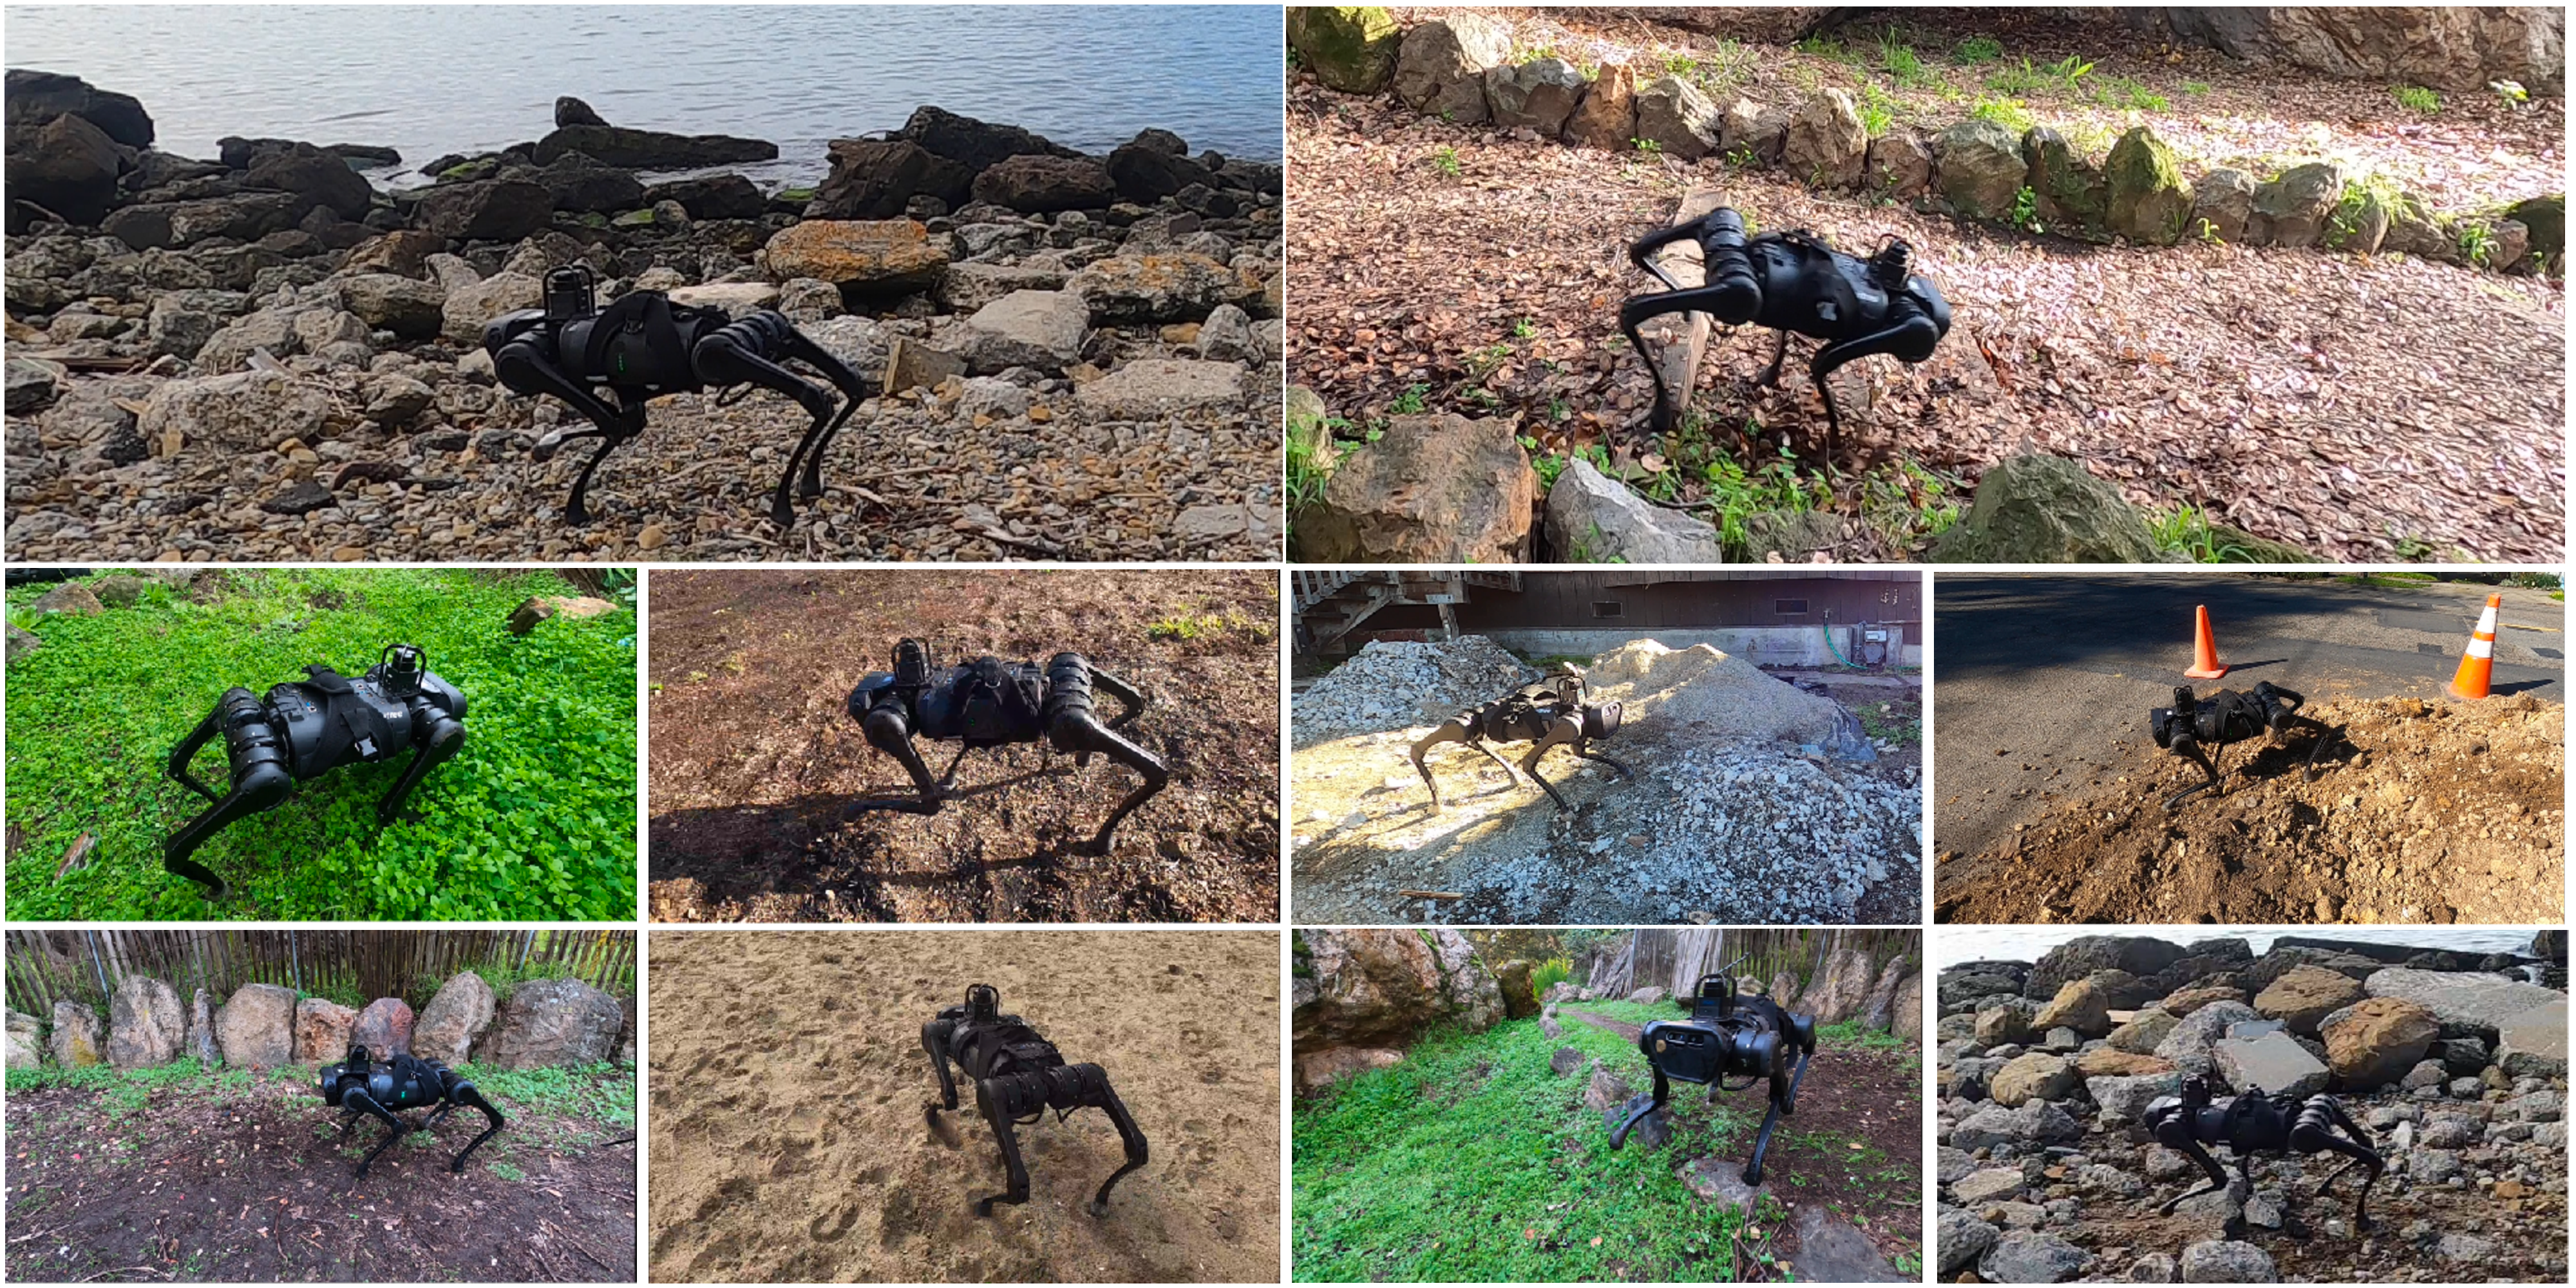
\includegraphics[width=0.72\textwidth,keepaspectratio]{outdoors-alt.pdf}

  \vspace{0.8mm}
  \raggedright
  {\small
  砂・泥・土，高い草や茂みは試行中の失敗なし．ハイキングコースの下り階段は 70\%．セメント片と砂利は 80\%．階段は訓練に無い．}

  \source{Kumar et al., Fig.~1, §5.2 \quad 動画：\url{https://ashish-kmr.github.io/rma-legged-robots/}}
\end{frame}

\begin{frame}{分析 ｜ 滑りは $\hat z$ の変化として残る}
  \begin{columns}[c,onlytextwidth]
    \begin{column}{0.40\textwidth}
      \begin{itemize}
        \item 約 2 秒で滑り始めると，歩容が乱れ，$\hat z$ の成分が動く．
        \item 回復後，トルクは少し大きく，周期は元に近い．
        \item $\hat z$ は元に戻らず，面がまだ滑ることを保持する．
      \end{itemize}
    \end{column}
    \begin{column}{0.58\textwidth}
      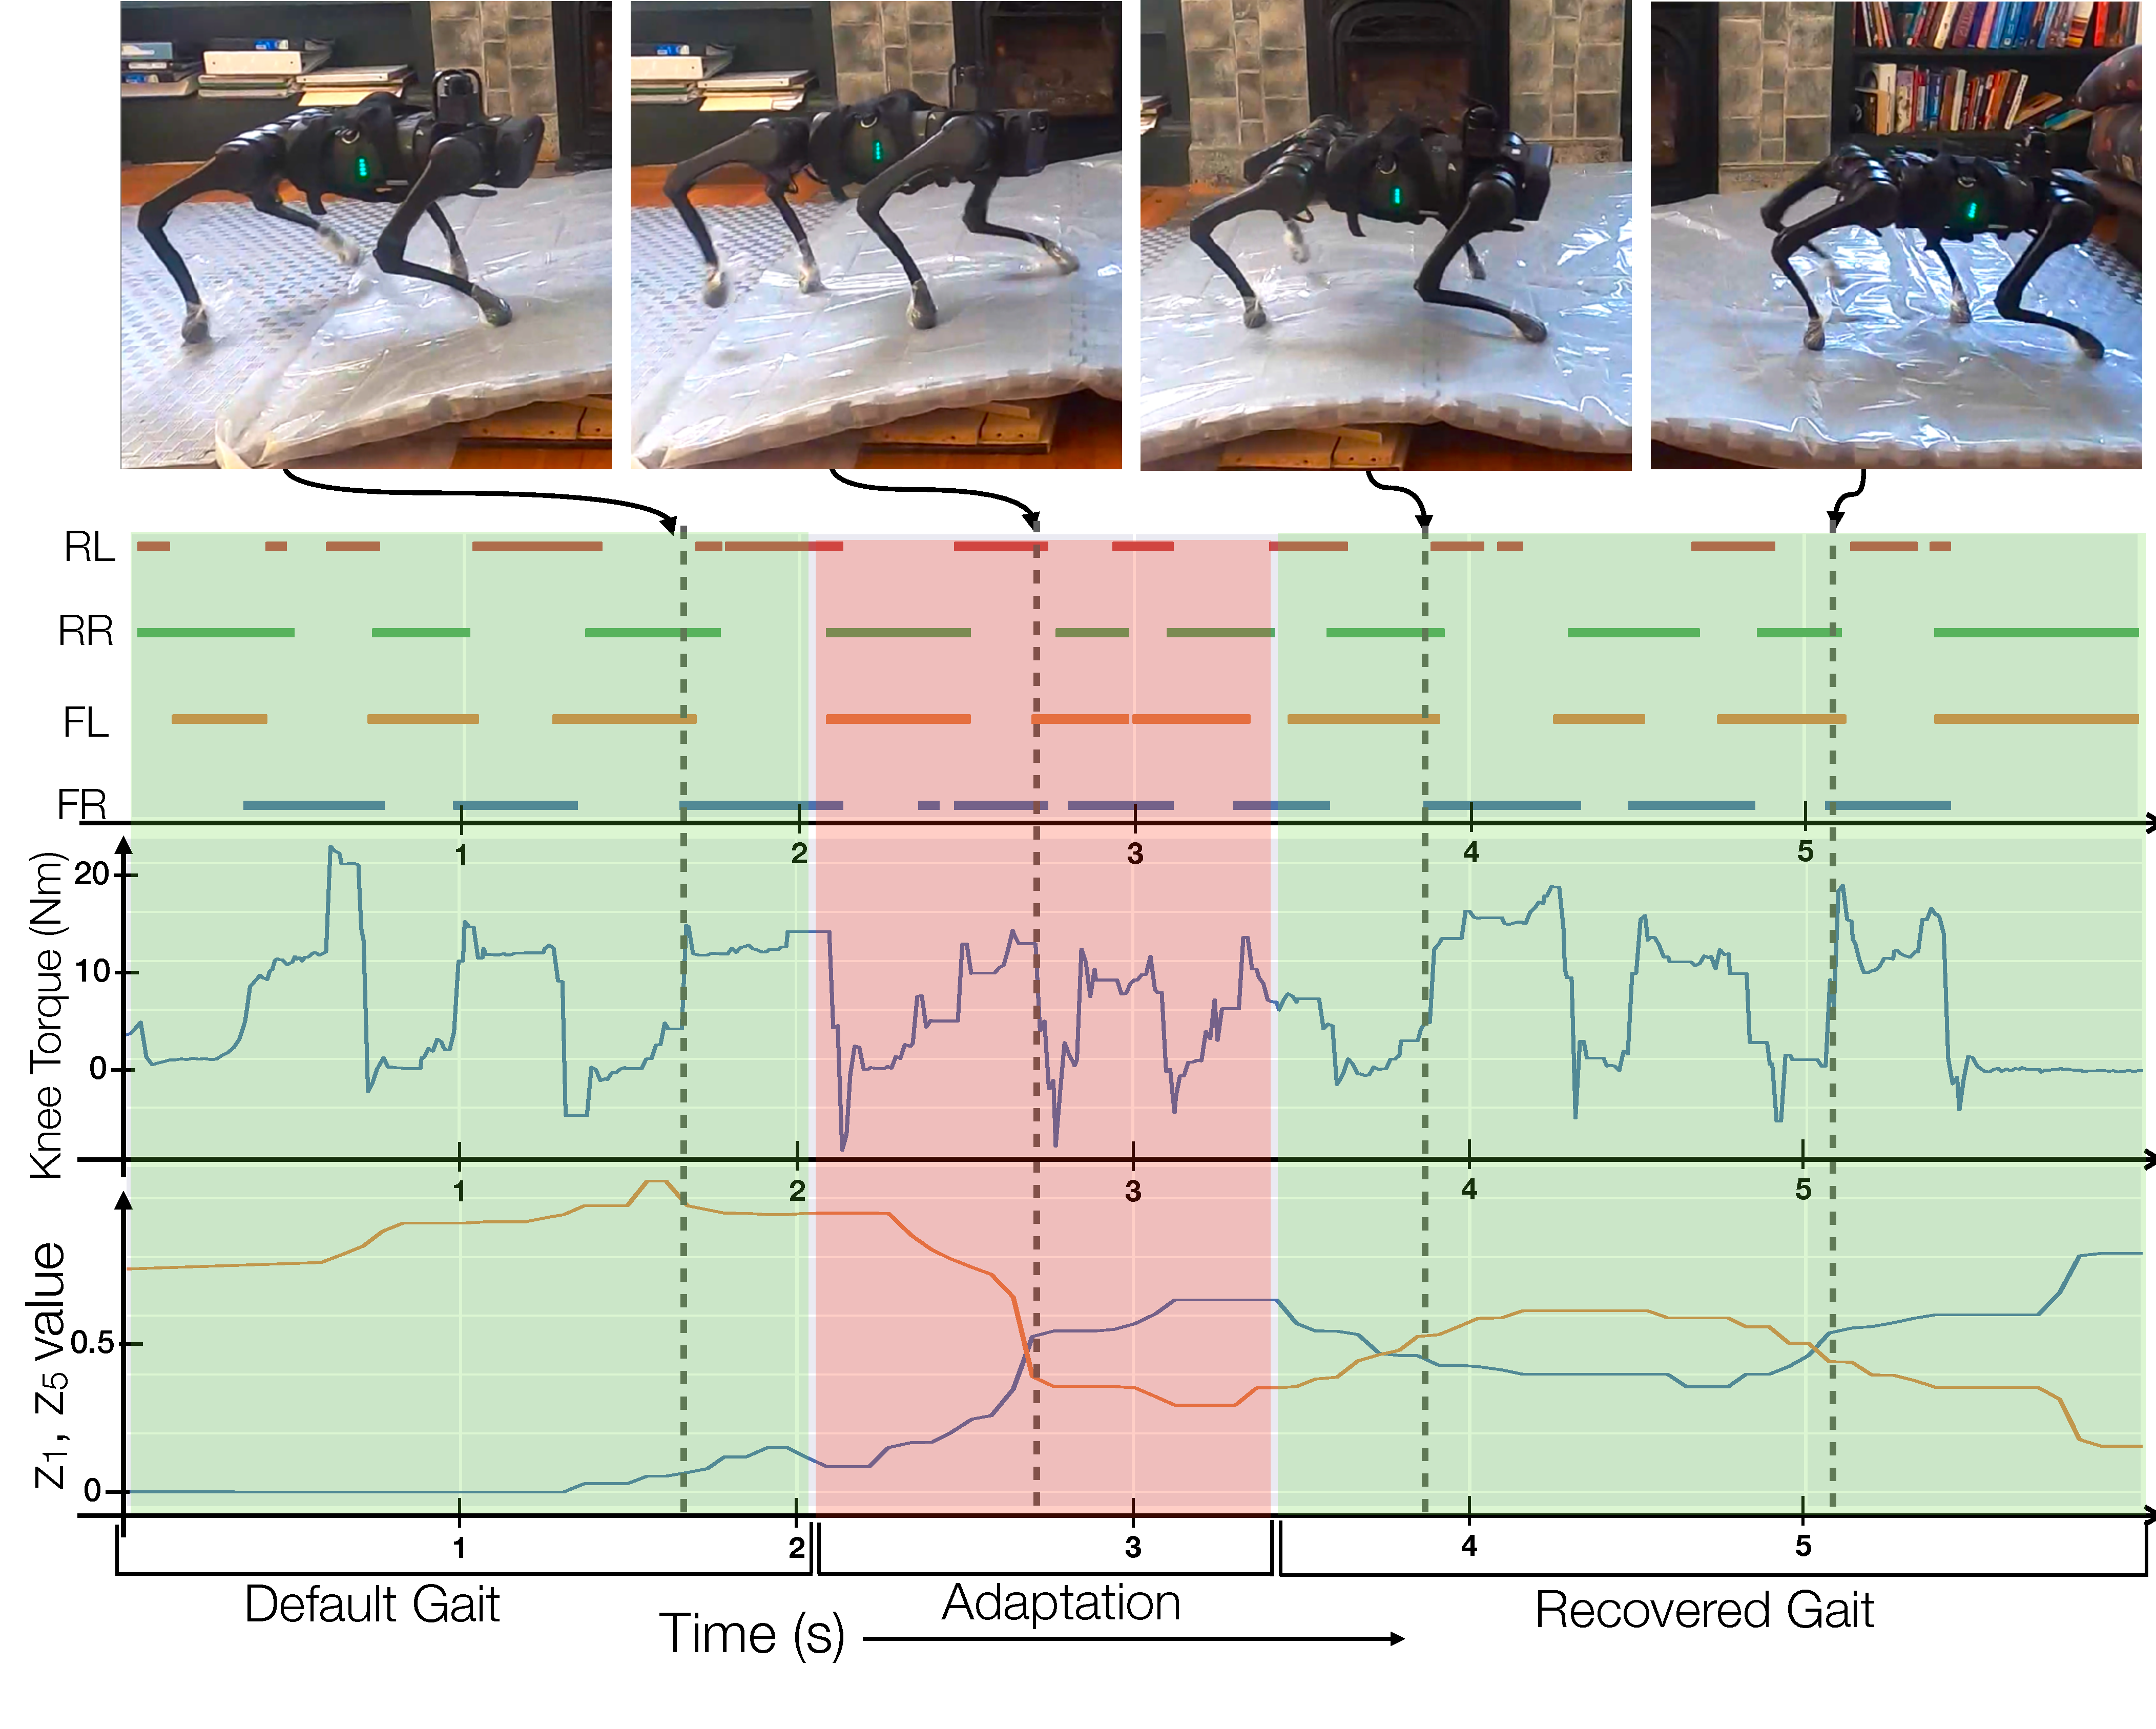
\includegraphics[height=46mm,keepaspectratio]{friction-analysis-fig.pdf}
    \end{column}
  \end{columns}
  \takeaway{推定した $\hat z$ は，歩き方を切り替える手がかりとして残っていれば足りる．}
  \source{Kumar et al., Fig.~4, §5.4 \quad 油のシートでの成功率は 90\%．}
\end{frame}

\begin{frame}{まとめ ｜ 適応を，実行時の最適化にしない}
  \begin{columns}[T,onlytextwidth]
    \begin{column}{0.32\textwidth}
      \infocard[orange]{学ぶこと}{特権情報 $e_t$ で方策を学び，実行時は 0.5 秒の履歴から $z_t$ を推定する．}
    \end{column}
    \hfill
    \begin{column}{0.32\textwidth}
      \infocard[green]{使わないもの}{参照軌道．実機での微調整．シミュレータの校正．}
    \end{column}
    \hfill
    \begin{column}{0.32\textwidth}
      \infocard[blue]{残る限界}{固有感覚のみ．大きな転倒や，複数の脚の引っかかりは失敗する．次は視覚．}
    \end{column}
  \end{columns}

  \vspace{0.9em}
  \centering
  \metricbox[orange]{73.5\%}{シミュレーション\\Expert は 76.2\%}\hspace{1.4em}%
  \metricbox[green]{砂・泥・草}{段差と，体重分の荷物}

  \takeaway{役立つ分担は，速い身体の制御と，遅い環境の推定を，別の周期で持つこと．}
  \source{Kumar et al., §6}
\end{frame}

\begin{frame}{文献}
  {\footnotesize
  \begin{enumerate}
    \item Kumar, Fu, Pathak, Malik.
      \textbf{RMA: Rapid Motor Adaptation for Legged Robots.}
      RSS 2021.\\
      \url{https://arxiv.org/abs/2107.04034}
      \quad
      \url{https://ashish-kmr.github.io/rma-legged-robots/}
    \item Peng et al. Learning Agile Robotic Locomotion Skills by Imitating Animals. RSS 2020.
    \item Lee et al. Learning Quadrupedal Locomotion over Challenging Terrain. Science Robotics, 2020.
    \item Hwangbo et al. Learning Agile and Dynamic Motor Skills for Legged Robots. Science Robotics, 2019.
    \item Yu et al. Preparing for the Unknown: Learning a Universal Policy with Online System Identification. RSS 2017.
    \item Tobin et al. Domain Randomization for Transferring Deep Neural Networks from Simulation to the Real World. IROS 2017.
  \end{enumerate}}
\end{frame}

\end{document}
